\documentclass[11pt, a4paper]{article}
\usepackage[margin=2.5cm]{geometry}
\usepackage{amsmath}
\usepackage{amssymb}
\usepackage{booktabs}
\usepackage{graphicx}
\usepackage{float}
\usepackage{hyperref}
\usepackage{xcolor}
\usepackage{titlesec}
\usepackage{parskip}
\usepackage{lmodern}
\usepackage{microtype}
\usepackage{caption}
\usepackage{array}
\usepackage{tabularx}

\hypersetup{
    colorlinks=true,
    linkcolor=black,
    urlcolor=black,
    citecolor=black
}

\titleformat{\section}
  {\large\bfseries}{\thesection}{1em}{}[\titlerule]
\titleformat{\subsection}
  {\normalsize\bfseries}{\thesubsection}{1em}{}

\definecolor{darkblue}{RGB}{44, 95, 138}

\begin{document}

\begin{titlepage}
\centering
\vspace*{3cm}
{\Huge\bfseries Market Risk Analysis \par}
\vspace{0.5cm}
{\Large VaR, Expected Shortfall \& Stress Testing \par}
\vspace{1cm}
\textcolor{darkblue}{\rule{0.6\textwidth}{1.5pt}}
\vspace{1cm}

{\large Mohammad Valizadehmoghadam \par}
\vspace{0.3cm}
{\normalsize Master of Financial Risk Management \par}
{\normalsize Rotman School of Management, University of Toronto \par}
\vspace{1cm}
{\normalsize April 2026 \par}

\vspace{2cm}
\begin{abstract}
\noindent
This report presents a full market risk measurement framework 
applied to a mixed long/short portfolio of equity, investment 
grade credit, high yield credit, and US Treasury instruments. 
The analysis covers instrument pricing under continuous 
compounding, first-order sensitivity analysis, historical 
simulation Value-at-Risk and Expected Shortfall over a 
two-year market data window spanning 2021 to 2022, VaR 
model backtesting, and stress testing under a severely 
adverse macro scenario. Supplementary analysis includes 
DV01 by tenor, risk factor correlation structure, and 
regulatory capital scaling under the Fundamental Review 
of the Trading Book. The portfolio is found to be 
predominantly a credit risk book despite its apparent 
diversification, with credit spread sensitivity 
approximately twelve times larger than rate sensitivity. 
Under a 2008-style stress scenario the portfolio loses 
\$410,371, forty-three times the statistical one-day VaR 
of \$9,485 --- a gap that illustrates the complementary 
role of scenario-based and statistical risk measures in 
modern risk management.
\end{abstract}
\end{titlepage}

\tableofcontents
\newpage

\section{Executive Summary}

This project implements a complete market risk measurement stack for a four-instrument portfolio combining equity, investment-grade credit, high-yield credit, and a short U.S.\ Treasury hedge. It prices positions under continuous compounding, derives first-order sensitivities, runs historical simulation for VaR and Expected Shortfall, and contrasts full revaluation with Taylor-based stress approximations.

The empirical results are economically large. The portfolio one-day 99\% Value-at-Risk is \$9,485 on the worst scenario date 2022-02-11. Expected Shortfall at the 97.5\% level is \$9,974, yielding an ES/VaR ratio of 1.05x. Under the severely adverse macro stress scenario the portfolio loses \$410,371 on a full revaluation basis, which is approximately forty-three times the statistical one-day VaR of \$9,485 and underscores how scenario losses can dwarf tail statistics calibrated to recent history.

The dominant risk insight is credit spread exposure. CS01 is \$1,007 per basis point versus PV01 of \$82 per basis point, so the book behaves predominantly as a credit risk portfolio despite surface diversification across asset classes. The short UST position hedges parallel rate moves but does not hedge credit spreads; in stress, the investment-grade bond alone drives about 65\% of total losses.

Formal VaR backtesting against the 99\% threshold shows breach counts consistent with the Basel III internal-models green zone under normal conditions. From a regulatory perspective, Basel III and the Fundamental Review of the Trading Book (FRTB) have shifted emphasis toward Expected Shortfall at 97.5\% as a tail-coherent replacement for standalone 99\% VaR in many capital frameworks.

\section{Portfolio Overview}

The portfolio holds a long equity ETF, long investment-grade and high-yield corporate bonds, and a short five-year U.S.\ Treasury intended as an explicit rate hedge against the rate-sensitive bond legs.

\begin{table}[H]
\centering
\caption{Portfolio Composition}
\begin{tabularx}{\textwidth}{lXXXX}
\toprule
\textbf{Instrument} & \textbf{Position} & 
\textbf{Size} & \textbf{Maturity} & 
\textbf{Coupon} \\
\midrule
SPY ETF & Long & 30 units & N/A & N/A \\
IG Corporate Bond (A) & Long & 10,000 & 
10yr & 5.00\% \\
HY Corporate Bond (BB) & Long & 10,000 & 
2yr & 7.00\% \\
US Treasury & Short & 20,000 & 5yr & 
3.875\% \\
\bottomrule
\end{tabularx}
\end{table}

\begin{table}[H]
\centering
\caption{Spot Market Data}
\begin{tabularx}{\textwidth}{lX}
\toprule
\textbf{Risk Factor} & \textbf{Value} \\
\midrule
SPY Price & \$380.82 \\
UST Yield @ 2yr & 4.25\% \\
UST Yield @ 5yr & 3.70\% \\
UST Yield @ 10yr & 3.56\% \\
IG Credit Spread (A) & 112 bps \\
HY Credit Spread (BB) & 295 bps \\
\bottomrule
\end{tabularx}
\end{table}

\section{Methodology}

\subsection{Analytical Framework}

The analysis chains together four building blocks. Fixed-income instruments are valued with continuously compounded discounting off the Treasury curve plus option-adjusted credit spreads where relevant. First-order rate and spread sensitivities are obtained by symmetric numerical perturbation in the pricing engine. Historical simulation revalues (or linearly approximates) the portfolio across 501 daily joint shocks from January 2021 through December 2022. Stress testing compares a full nonlinear repricing to a first-order Taylor expansion under a single severely adverse scenario. The 501-day window is the empirical backbone for VaR, ES, shock histograms, and backtesting.

\subsection{Risk Measures}

Value-at-Risk (VaR) summarizes the loss threshold exceeded only rarely at a chosen confidence level; Expected Shortfall (ES) averages losses beyond that VaR threshold and therefore describes the depth of the left tail rather than a single quantile. PV01 measures the dollar change in present value for a one basis point parallel shift in Treasury yields, while CS01 isolates the same for a one basis point widening in the credit spread component holding the Treasury curve fixed. Equity delta here denotes the portfolio P\&L associated with a one percent move in the SPY price. DV01 generalizes rate sensitivity to specific curve tenors rather than a single parallel factor. Full revaluation reprices each instrument under stressed inputs; the Taylor approximation linearizes the P\&L using the pre-shock sensitivities and is useful for diagnostics but can diverge for large yield moves.

\section{Instrument Pricing}

Bond present values are computed by discounting each semi-annual coupon and the principal repayment at continuously compounded yields that sum the risk-free Treasury rate and the credit spread for corporate bonds.

\begin{equation}
PV = \sum_{i=1}^{n} C \cdot e^{-r \cdot t_i} 
+ F \cdot e^{-r \cdot T}
\end{equation}

Where $C$ is the coupon payment per period, $F$ 
is the face value, $r$ is the continuously compounded discount rate (risk-free yield plus 
credit spread), $t_i$ is the time to the $i$-th cash flow, and $T$ is the time to maturity.

\begin{table}[H]
\centering
\caption{Present Values per Position}
\begin{tabularx}{\textwidth}{lXX}
\toprule
\textbf{Instrument} & \textbf{Discount Rate} & 
\textbf{Present Value} \\
\midrule
SPY ETF & N/A (market price) & \$380.82 \\
IG Corporate Bond & 3.56\% + 1.12\% = 4.68\% & 
\$102.09 \\
HY Corporate Bond & 4.25\% + 2.95\% = 7.20\% & 
\$99.39 \\
US Treasury & 3.70\% & \$100.64 \\
\bottomrule
\end{tabularx}
\end{table}

Per unit of face (or one share for SPY), the IG bond trades above par because its coupon exceeds its discount rate, the HY bond trades just below par because the coupon sits just under the all-in discount rate, and the Treasury prices just above par against the five-year continuously compounded yield.

\section{Risk Sensitivities}

Sensitivities are computed by bumping the relevant risk factor, repricing, and differencing against the base case---a standard numerical derivative that avoids hand-derived bond Greeks while staying consistent with the pricing code.

\begin{equation}
\text{Sensitivity} = PV(r + \varepsilon) - PV(r)
\end{equation}

Where $\varepsilon = 0.0001$ (1 basis point) for 
PV01 and CS01, and 1\% for Equity Delta.

\begin{table}[H]
\centering
\caption{First-Order Sensitivities}
\begin{tabularx}{\textwidth}{lXX}
\toprule
\textbf{Sensitivity} & \textbf{Shock} & 
\textbf{Portfolio P\&L} \\
\midrule
Equity Delta & +1\% SPY price & +\$114.25 \\
PV01 & +1 bps parallel rate shift & --\$82.05 \\
CS01 & +1 bps credit spread widening & 
--\$1,006.65 \\
\bottomrule
\end{tabularx}
\end{table}

In absolute terms CS01 is roughly twelve times PV01, which is the clearest quantitative signature that credit spread risk, not parallel rates, dominates the risk budget. Equity delta is modest relative to spread DV01, consistent with a bond-heavy construction.

\section{Historical Shock Analysis}

Each of the 501 scenarios applies the historical daily change in risk factors observed between 2021 and 2022. SPY shocks are relative returns; Treasury yields and credit spreads use absolute changes measured in basis points. The sample window captures the Federal Reserve hiking cycle, so rate and spread innovations exhibit volatility clustering and fat tails compared with calmer regimes.

\begin{figure}[H]
\centering
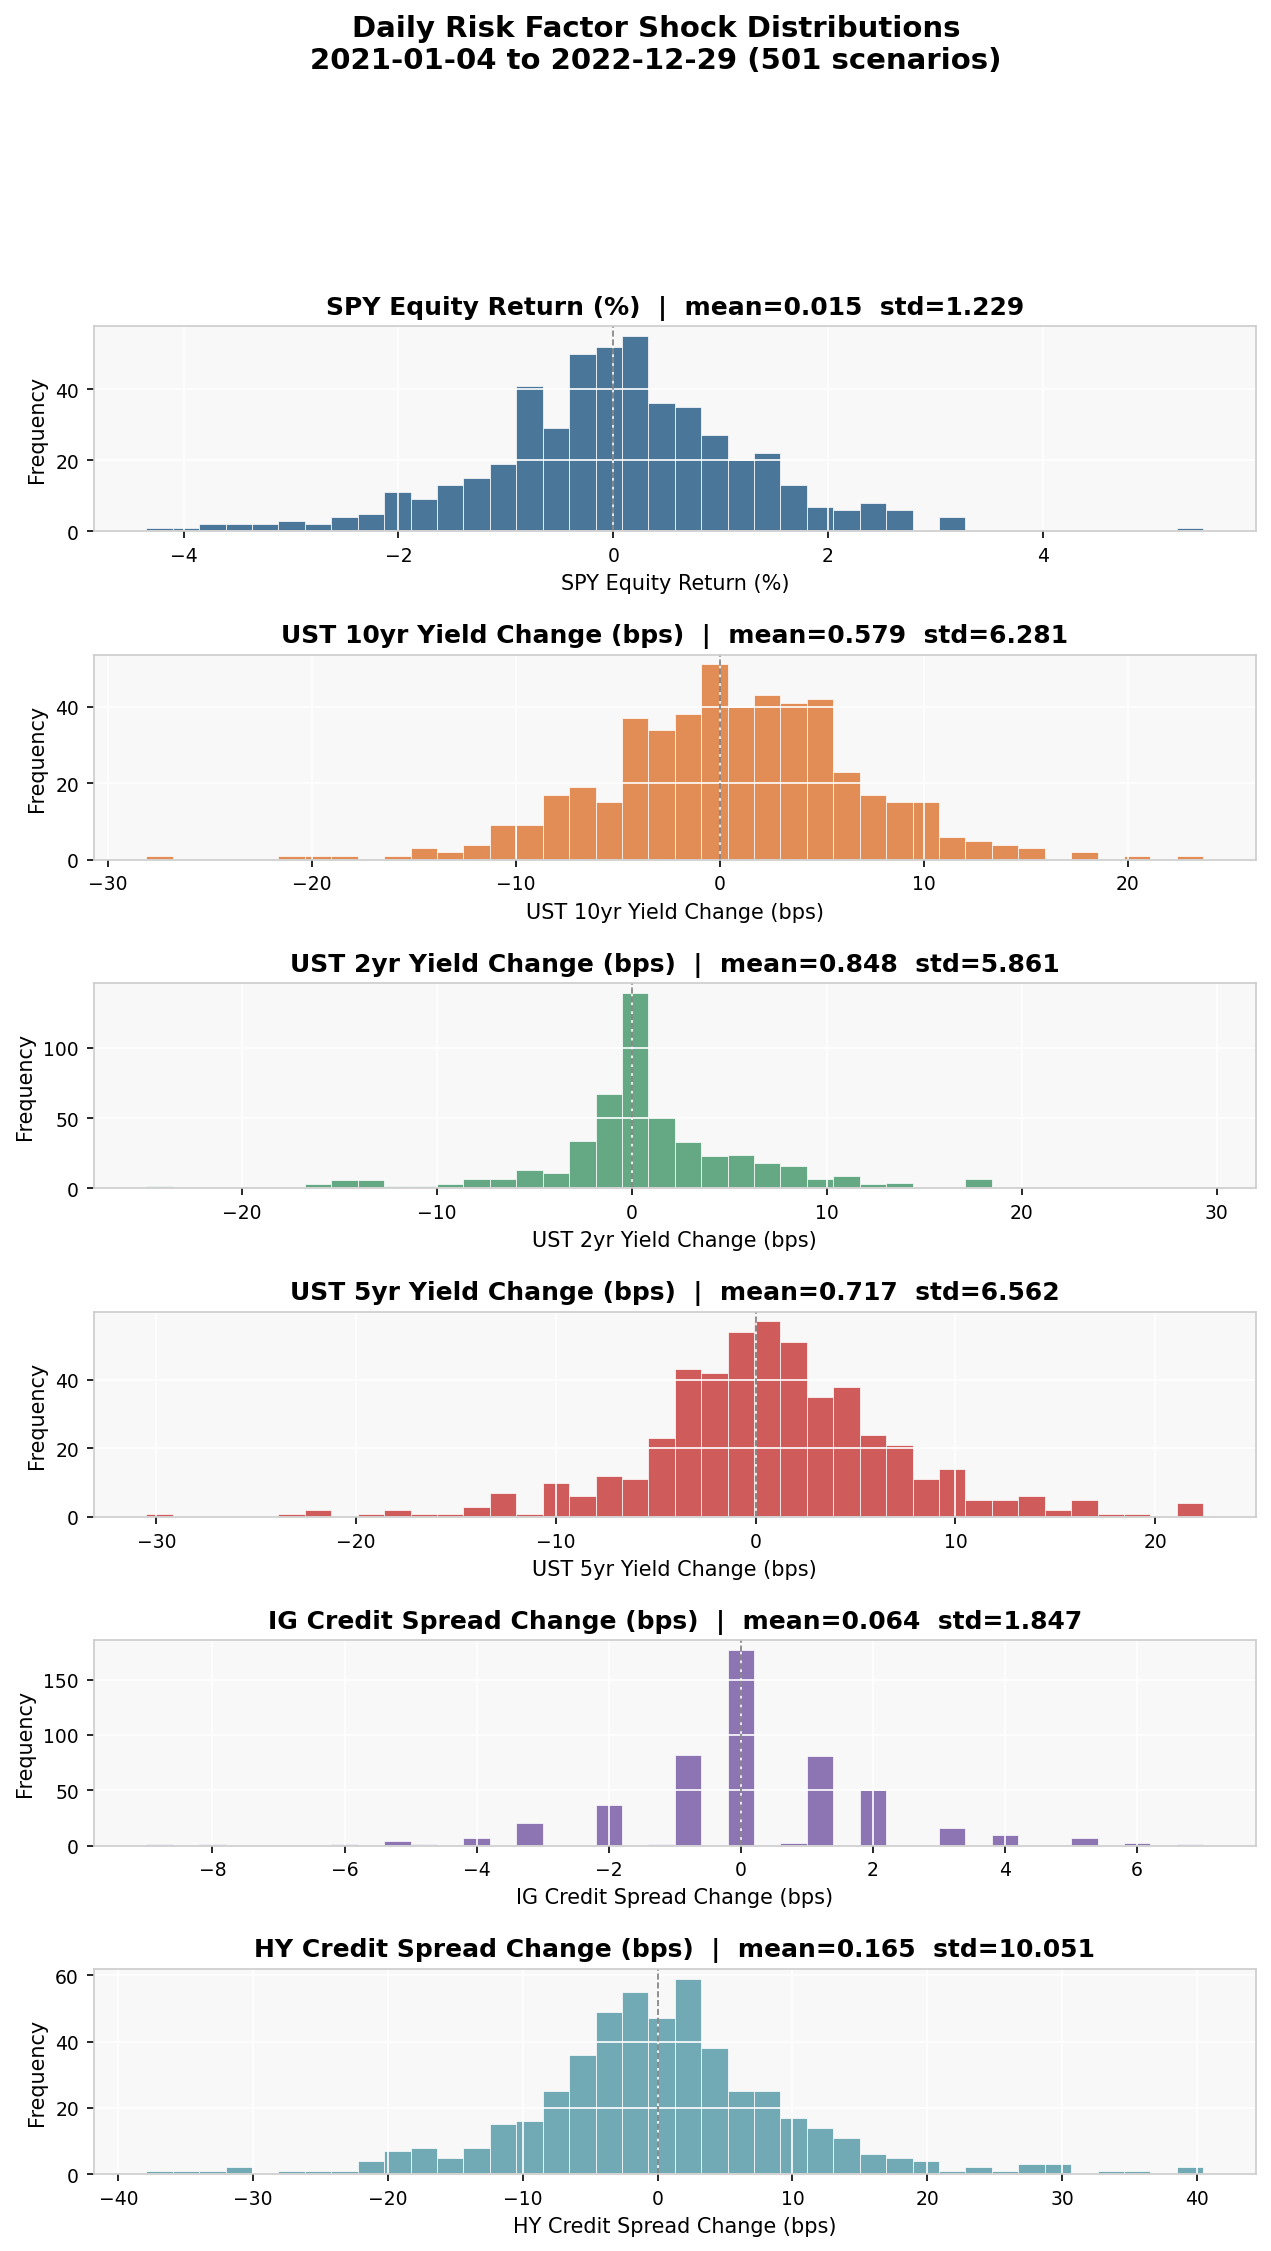
\includegraphics[width=0.85\textwidth]
{../output/daily_shock_histogram.png}
\caption{Daily risk factor shock distributions 
across 501 historical scenarios (2021--2022).}
\end{figure}

The histograms show roughly symmetric equity shocks, wider tails for Treasury yields consistent with a policy transition period, and the highest dispersion among credit factors in high yield spreads, reflecting episodic risk-off widening in that segment.

\section{Value-at-Risk and Expected Shortfall}

\subsection{Methodology}

For computational efficiency the historical P\&L distribution is built from a first-order Taylor expansion in the shocks, using sensitivities evaluated at the base market:

\begin{equation}
\Delta PV \approx \Delta_{\text{equity}} 
\cdot \delta_{\text{SPY}} + PV01 \cdot 
\delta_{r} + CS01 \cdot \delta_{cs}
\end{equation}

With 501 scenarios, the one-day 99\% VaR is the sixth worst loss because one percent of 501 equals 5.01 scenarios in the tail. The 97.5\% ES averages the thirteen worst losses because 2.5\% of 501 equals 12.525, which rounds up to thirteen tail observations.

\subsection{Results}

\begin{figure}[H]
\centering
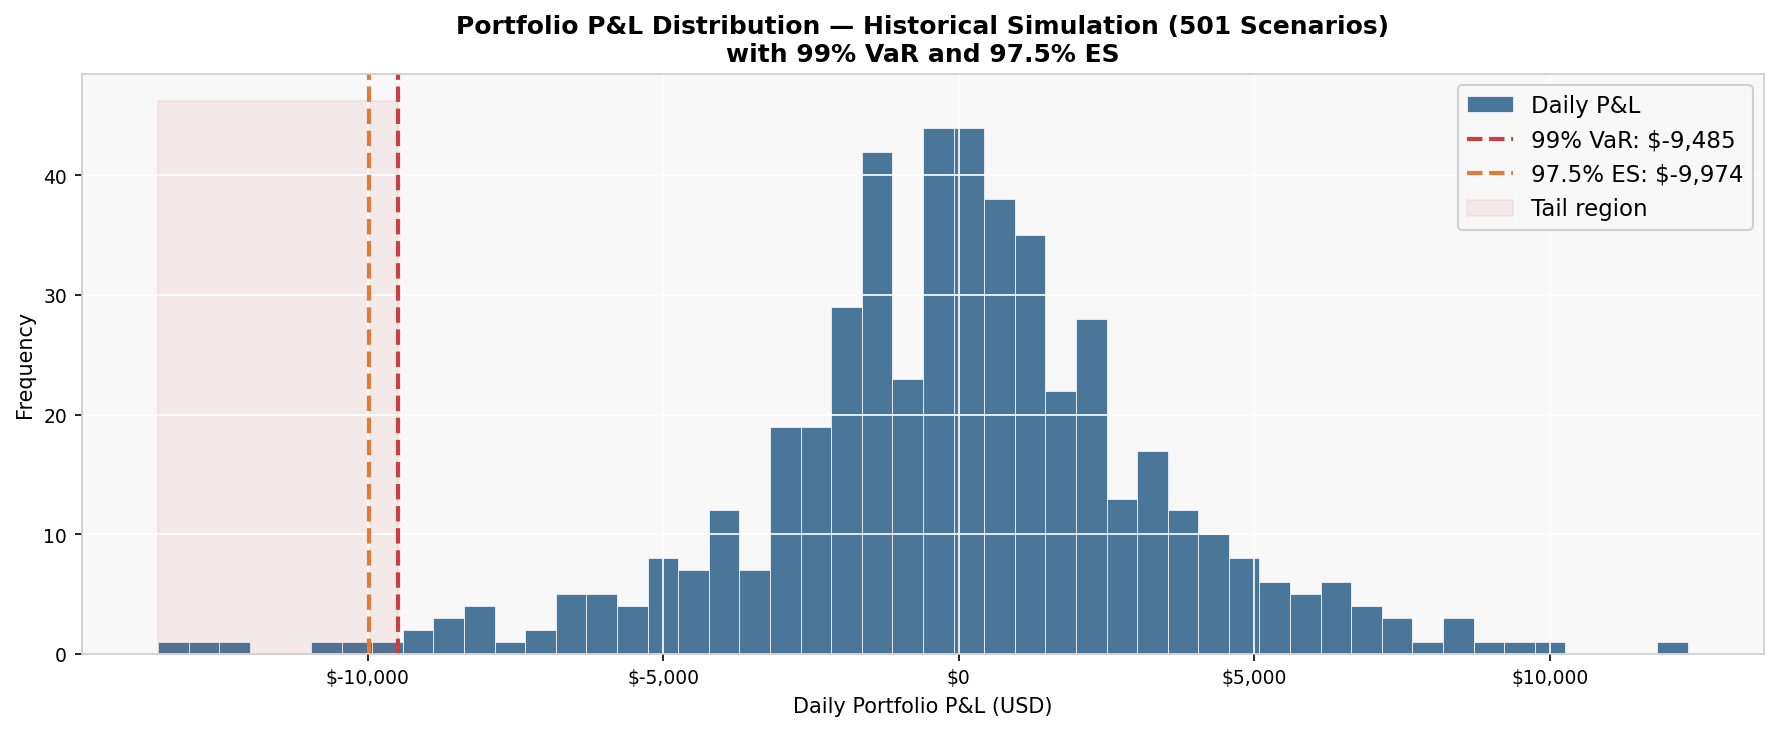
\includegraphics[width=\textwidth]
{../output/pnl_distribution.png}
\caption{Portfolio P\&L distribution across 
501 scenarios with 99\% VaR and 97.5\% ES.}
\end{figure}

\begin{table}[H]
\centering
\caption{VaR and ES Results}
\begin{tabularx}{\textwidth}{lXX}
\toprule
\textbf{Instrument} & \textbf{99\% VaR} & 
\textbf{Scenario Date} \\
\midrule
SPY ETF & --\$387 & 2022-08-26 \\
IG Corporate Bond & --\$13,084 & 2022-03-14 \\
HY Corporate Bond & --\$5,602 & 2022-09-13 \\
US Treasury & --\$16,920 & 2021-11-26 \\
Portfolio & --\$9,485 & 2022-02-11 \\
\midrule
\textbf{ES 97.5\%} & \multicolumn{2}{l}
{--\$9,974 (average of 13 worst scenarios)} \\
\bottomrule
\end{tabularx}
\end{table}

The portfolio VaR peaks on 2022-02-11, a session associated with a hot CPI print and correlated shocks across rates, spreads, and equity that the linear sensitivities translate into a large one-day loss. Component VaR dates differ because each leg responds to its own worst historical shock bundle.

The ES/VaR ratio of 1.05x indicates only modest tail severity beyond the 99\% quantile---losses worse than VaR are not dramatically larger on average. The UST leg's worst day (2021-11-26) reflects the short bond losing when yields fell sharply on Omicron-related flight-to-quality flows.

\section{VaR Backtesting}

Backtesting compares ex ante VaR estimates to realized (or historically simulated) P\&L outcomes, providing a simple reality check on whether the stated confidence level is roughly matched by empirical breach frequencies. Under the Basel III internal model traffic light approach for 500 observations at 99\% VaR, up to nine breaches defines the green zone, ten to twelve breaches define yellow, and more than twelve breaches trigger red.

\begin{figure}[H]
\centering
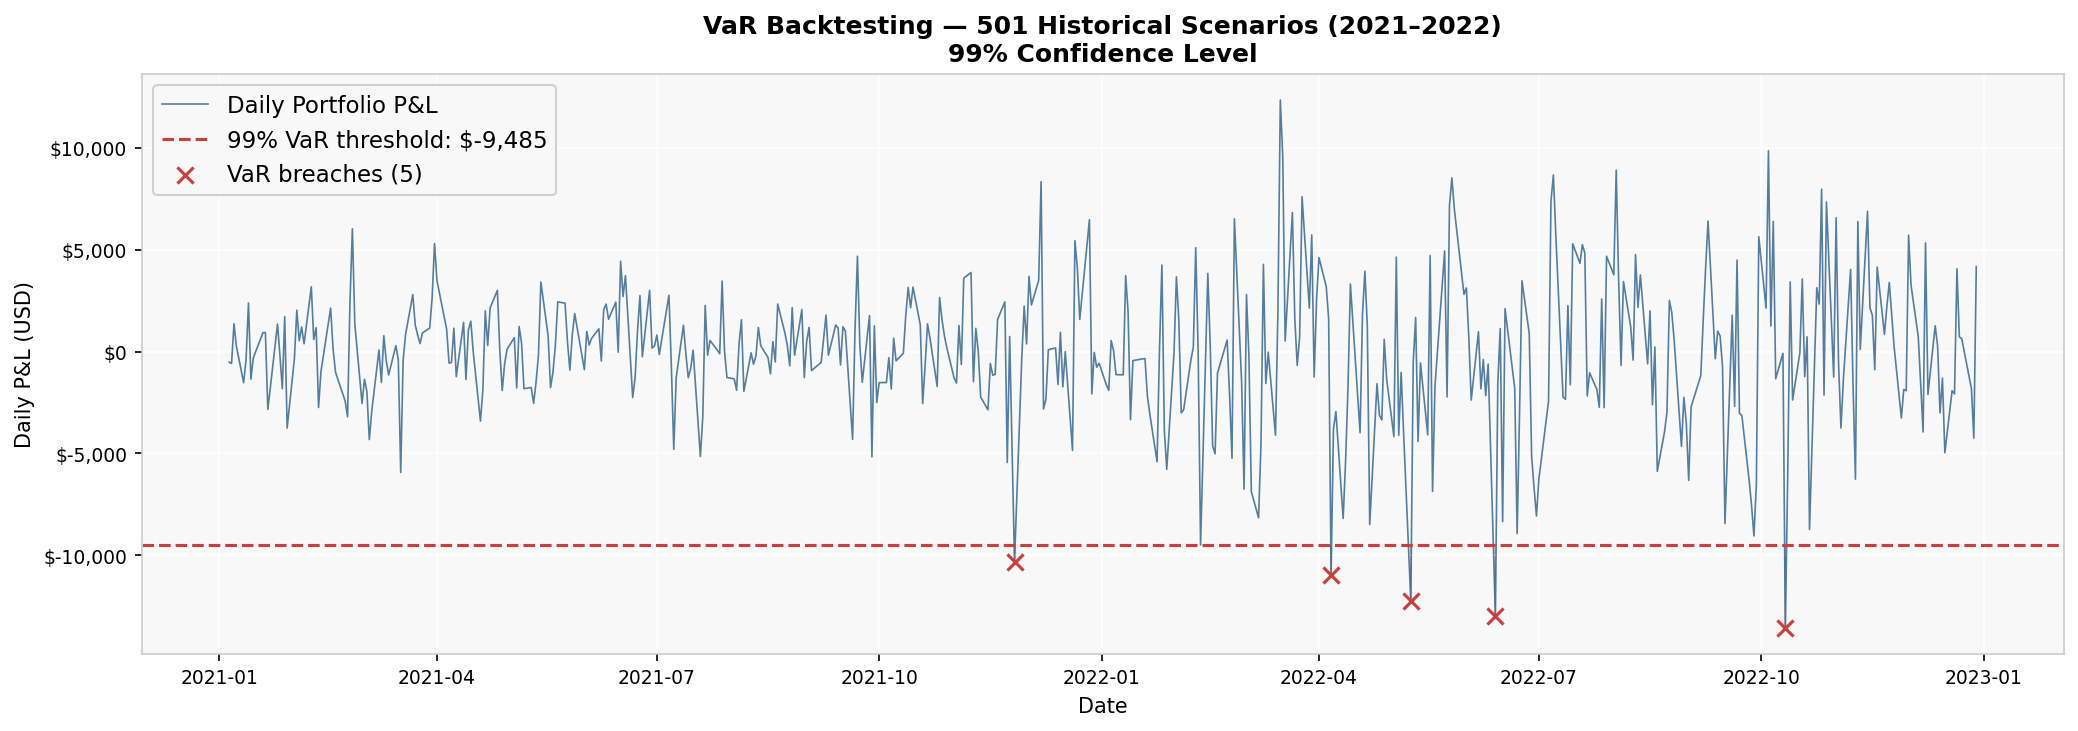
\includegraphics[width=\textwidth]
{../output/var_backtesting.png}
\caption{VaR backtesting: daily portfolio P\&L 
vs 99\% VaR threshold across 501 scenarios.}
\end{figure}

The exercise records five breaches of the 99\% VaR threshold across the 501 scenarios, which falls comfortably in the Basel III green zone (up to nine breaches). That outcome is consistent with a historical simulation engine whose breach frequency is close to the theoretical expectation of roughly one percent under the 2021--2022 experience.

\section{Stress Testing}

\subsection{Scenario Definition}

The severely adverse scenario applies simultaneous equity crash, Treasury bear steepening, and aggressive widening in investment-grade and high-yield spreads calibrated to a 2008-style macro shock.

\begin{table}[H]
\centering
\caption{Severely Adverse Stress Scenario}
\begin{tabularx}{\textwidth}{lX}
\toprule
\textbf{Risk Factor} & \textbf{Shock} \\
\midrule
SPY equity price & --38.3\% \\
UST yield @ 2yr & +29.9 bps \\
UST yield @ 5yr & +42.3 bps \\
UST yield @ 10yr & +49.4 bps \\
IG credit spread (A rating) & +337.6 bps \\
HY credit spread (BB rating) & +1,012.0 bps \\
\bottomrule
\end{tabularx}
\end{table}

\subsection{Full Revaluation vs Taylor}

Full revaluation feeds stressed curves and spreads through the bond pricing formulas and reprices each cash flow stream from scratch. The Taylor approximation applies only first-order sensitivities and therefore omits convexity with respect to yields and spreads. For large upward shifts in yields, bonds exhibit positive convexity: actual prices fall more slowly than the linear tangent predicts, so the Taylor path tends to overstate losses relative to full repricing.

\begin{table}[H]
\centering
\caption{Stress Testing Results: Full 
Revaluation vs Taylor Approximation}
\begin{tabularx}{\textwidth}{lXX}
\toprule
\textbf{Instrument} & \textbf{Full Reval} & 
\textbf{Taylor} \\
\midrule
SPY ETF & --\$4,376 & --\$4,376 \\
IG Corporate Bond & --\$266,660 & --\$316,477 \\
HY Corporate Bond & --\$178,057 & --\$196,792 \\
US Treasury (Short) & +\$38,722 & +\$39,110 \\
\midrule
\textbf{Portfolio} & \textbf{--\$410,371} & 
\textbf{--\$478,534} \\
\bottomrule
\end{tabularx}
\end{table}

\begin{figure}[H]
\centering
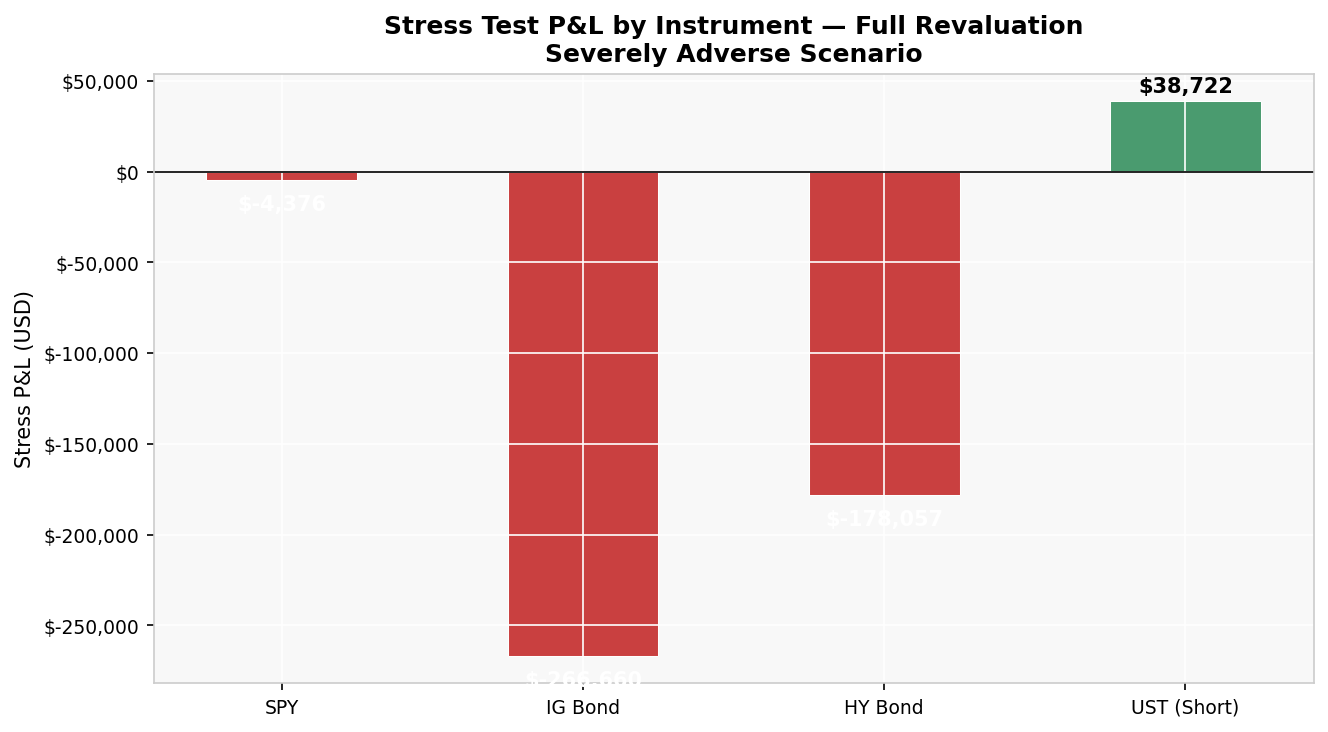
\includegraphics[width=0.9\textwidth]
{../output/stress_contribution.png}
\caption{Stress P\&L by instrument under full 
revaluation.}
\end{figure}

Under full revaluation the portfolio loses \$410,371, driven overwhelmingly by the long IG corporate position (about 65\% of the total), with additional HY losses partially offset by gains on the short Treasury hedge. The hedge works as designed for rates but cannot offset the credit widening that dominates the scenario.

Taylor understates convexity and therefore overstates the loss by \$68,163 (16.6\%) at the portfolio level relative to full revaluation. For regulatory and management stress reporting, full revaluation should always be preferred when systems capacity allows.

\section{Risk Limits Framework}

A three-layer limit stack is proposed: statistical tail limits (VaR), scenario loss caps, and granular sensitivity limits on equity delta, PV01, and CS01. The structure mirrors common desk practice where VaR caps overall tail risk, stress limits guard against narrative shocks absent from recent samples, and sensitivity limits catch incremental risk build before it appears in either statistical measure.

\begin{table}[H]
\centering
\caption{Proposed Risk Limits}
\begin{tabularx}{\textwidth}{lXXX}
\toprule
\textbf{Limit Type} & \textbf{Limit} & 
\textbf{Current} & \textbf{Headroom} \\
\midrule
VaR (1-day, 99\%) & \$15,000 & \$9,485 & 
\$5,515 \\
Stress Loss & \$500,000 & \$410,371 & 
\$89,629 \\
Equity Delta & \$500 & \$114 & \$386 \\
PV01 (per bps) & \$200 & \$82 & \$118 \\
CS01 (per bps) & \$1,500 & \$1,007 & \$493 \\
\bottomrule
\end{tabularx}
\end{table}

Among the sensitivity limits CS01 retains the least headroom (\$493 versus larger cushions on PV01 and equity delta), confirming that credit spread risk is the binding constraint despite the presence of an explicit rate hedge. The framework aligns with Basel III internal models practice where both tail statistics and sensitivities feed limit governance.

\section{DV01 by Tenor}

DV01 here means the dollar P\&L for a one basis point move in the specific Treasury tenor that anchors each instrument's discounting, rather than a single parallel shift across the entire curve. Decomposing DV01 by tenor clarifies where duration is concentrated along the curve and whether hedges such as the five-year short offset the dominant exposures.

\begin{table}[H]
\centering
\caption{DV01 by Tenor Bucket}
\begin{tabularx}{\textwidth}{lXX}
\toprule
\textbf{Tenor} & \textbf{Instrument} & 
\textbf{DV01 (per bps)} \\
\midrule
2yr & HY Corporate Bond & --\$188.88 \\
5yr & US Treasury (Short) & +\$924.60 \\
10yr & IG Corporate Bond & --\$817.77 \\
\bottomrule
\end{tabularx}
\end{table}

The ten-year bucket dominates through the long IG bond, the five-year short Treasury provides partial offsetting positive DV01, and the two-year HY contribution is smaller in magnitude but reinforces the net short-rate position at the front end.

\section{Risk Factor Correlations}

The correlation matrix over daily shocks shows Treasury yields across two-, five-, and ten-year tenors moving together with strongly positive coefficients, consistent with quasi-parallel shifts during a hiking cycle. SPY returns exhibit moderate negative correlation with yield changes, capturing a partial risk-off relationship between equities and rates. Investment-grade and high-yield credit spreads move positively with each other but only weakly with rate levels, implying that rate and credit factors are relatively independent in this window---so the short Treasury hedge mitigates one factor class without insulating the portfolio from spread widening.

\section{FRTB and Liquidity Horizons}

\subsection{Regulatory Context}

The Fundamental Review of the Trading Book is the Basel Committee's overhaul of market risk capital requirements, finalized in 2019 and being implemented by major jurisdictions through the mid-2020s. It replaced Value-at-Risk with Expected Shortfall as the primary risk measure, moving from a 99\% confidence VaR to a 97.5\% ES, which better captures tail risk and satisfies coherence properties such as subadditivity that VaR can violate.

Under FRTB's internal models approach, different risk factor classes carry minimum liquidity horizons reflecting how long it takes to hedge or exit positions under stress. Horizons range from ten days for large-cap equity to sixty days for high-yield credit spreads, embedding liquidity into the capital multiplier.

\subsection{Liquidity Horizon Scaling}

A common illustrative scaling from one day to $T$ days assumes i.i.d.\ shocks and uses the square-root-of-time rule:

\begin{equation}
VaR(T) = VaR(\text{1-day}) \times \sqrt{T}
\end{equation}

This is illustrative only: FRTB's internal models approach uses ES, not VaR, and applies liquidity horizons at the risk-factor level with more elaborate dependence than a single scalar scaling.

\begin{table}[H]
\centering
\caption{FRTB Liquidity Horizon Scaling}
\begin{tabularx}{\textwidth}{lXXXX}
\toprule
\textbf{Instrument} & \textbf{Risk Class} & 
\textbf{Horizon} & \textbf{1-day VaR} & 
\textbf{Scaled VaR} \\
\midrule
SPY & Equity & 10 days & --\$387 & 
--\$1,223 \\
IG Bond & IG Credit & 40 days & --\$13,084 & 
--\$82,753 \\
HY Bond & HY Credit & 60 days & --\$5,602 & 
--\$43,395 \\
UST (Short) & Rates & 20 days & --\$16,920 & 
--\$75,669 \\
\bottomrule
\end{tabularx}
\end{table}

The IG bond's scaled VaR grows sharply because a large standalone 99\% VaR is multiplied by the square root of a forty-day liquidity horizon, illustrating why FRTB assigns longer horizons to less liquid credit instruments than to large-cap equities.

\section{Key Takeaways}

The portfolio is a credit risk book in disguise. Although it holds four instruments spanning equity, government rates, and corporate credit, CS01 of \$1,007 per basis point dwarfs PV01 of \$82, so day-to-day P\&L volatility is dominated by spread moves rather than parallel Treasury shifts.

The short UST hedge is partial at best. It offsets rate risk effectively---delivering roughly +\$38,722 in the severely adverse scenario---but provides essentially no insulation against the credit spread widening that drives the bulk of stress losses.

VaR and stress testing are complements, not substitutes. The forty-three-fold gap between \$9,485 VaR and \$410,371 stress loss is not evidence that either tool is wrong; VaR summarizes tail behavior within the empirical window while stress testing probes structured extremes outside that window, and modern risk governance requires both lenses.

Full revaluation is always preferred for large shocks. The Taylor approximation overstated the portfolio loss by \$68,163 (16.6\%) because it ignores bond convexity; when shocks are large relative to typical daily moves, repricing from first principles is the only reliable approach.

\end{document}
